

\section{Nhóm Tính Năng Đăng Ký và Đăng Nhập}
\label{sec:impl_auth}

Nhóm tính năng đăng ký và đăng nhập cung cấp giao diện để người dùng truy cập hệ thống, đảm bảo bảo mật và trải nghiệm cá nhân hóa. Các màn hình được thiết kế đơn giản, thân thiện, hỗ trợ người dùng dễ dàng tạo tài khoản hoặc đăng nhập để sử dụng các tính năng chính.

\subsection{Giao Diện Trang Chủ}
\label{subsec:impl_ui_home}
Giao diện trang chủ hiển thị tổng quan hệ thống, bao gồm thông tin hệ thống, các tính năng hệ thống,... Người dùng có thể điều hướng đến các chức năng chính như đăng ký, đăng nhập, hoặc khám phá các tính năng.

\begin{figure}[H]
    \centering
    
\includegraphics[width=0.8\textwidth]{Images/trangchu.jpg}
    \vspace{1.5em}
    \caption{Giao diện trang chủ hệ thống}
    \label{fig:ui_home}
\end{figure}

\subsection{Giao Diện Trang Đăng Ký}
\label{subsec:impl_ui_register}
Giao diện đăng ký cho phép người dùng tạo tài khoản mới bằng cách nhập thông tin như email, mật khẩu, và tên người dùng. Các trường nhập liệu được thiết kế rõ ràng, kèm thông báo lỗi để hướng dẫn người dùng.

\begin{figure}[H]
    \centering
    
\includegraphics[width=0.8\textwidth]{Images/dangky.jpg}
    \vspace{1.5em}
    \caption{Giao diện trang đăng ký}
    \label{fig:ui_register}
\end{figure}

\subsection{Giao Diện Trang Đăng Nhập}
\label{subsec:impl_ui_login}
Giao diện đăng nhập yêu cầu người dùng nhập email và mật khẩu. Tùy chọn "Quên mật khẩu" và liên kết đến trang đăng ký được tích hợp để tăng tiện lợi.

\begin{figure}[H]
    \centering
    
\includegraphics[width=0.8\textwidth]{Images/dangnhap.jpg}
    \vspace{1.5em}
    \caption{Giao diện trang đăng nhập}
    \label{fig:ui_login}
\end{figure}
\newpage
\section{Tính Năng Cộng Đồng}
\label{sec:impl_community}

Tính năng cộng đồng cho phép người dùng xem, tương tác, và chia sẻ các bài viết. Đồng thời theo dõi được thực đơn, sự kiện, hoặc thử thách mà người dùng đang tham gia. Giao diện hiển thị danh sách bài viết từ cộng đồng, hỗ trợ các tính năng liên quan.

\begin{figure}[H]
    \centering
    
\includegraphics[width=0.8\textwidth]{Images/congdong.jpg}
    \vspace{1.5em}
    \caption{Giao diện trang cộng đồng}
    \label{fig:ui_community}
\end{figure}
\newpage
\section{Nhóm Tính Năng Thực Đơn}
\label{sec:impl_meal}

Nhóm tính năng thực đơn hỗ trợ người dùng tạo, quản lý, và chia sẻ thực đơn dinh dưỡng. Các giao diện được thiết kế trực quan, giúp người dùng dễ dàng lập kế hoạch bữa ăn và theo dõi lịch ăn uống.

\subsection{Giao Diện Trang Danh Sách Thực Đơn}
\label{subsec:impl_ui_meal_list}
Hiển thị danh sách các bài viết thực đơn từ cộng đồng hoặc người dùng đã lưu, hỗ trợ tìm kiếm và lọc theo thời gian hoặc danh mục.

\begin{figure}[H]
    \centering
    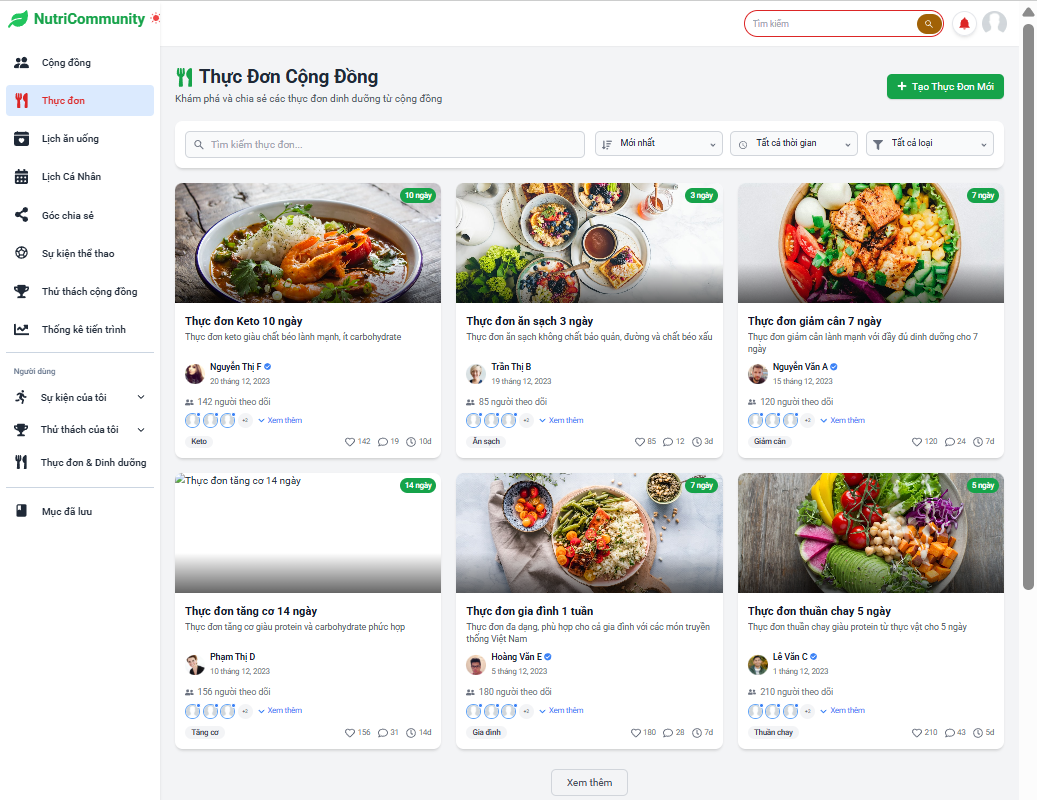
\includegraphics[width=0.8\textwidth]{Images/thucdon.jpg}
    \vspace{1.5em}
    \caption{Giao diện trang danh sách thực đơn}
    \label{fig:ui_meal_list}
\end{figure}

\subsection{Giao Diện Trang Tạo Thực Đơn}
\label{subsec:impl_ui_create_meal}
Cung cấp các trường để người dùng nhập thông tin thực đơn, bao gồm thời gian, món ăn, công thức, và hình ảnh. Hỗ trợ chọn món ăn có sẵn.

\begin{figure}[H]
    \centering
    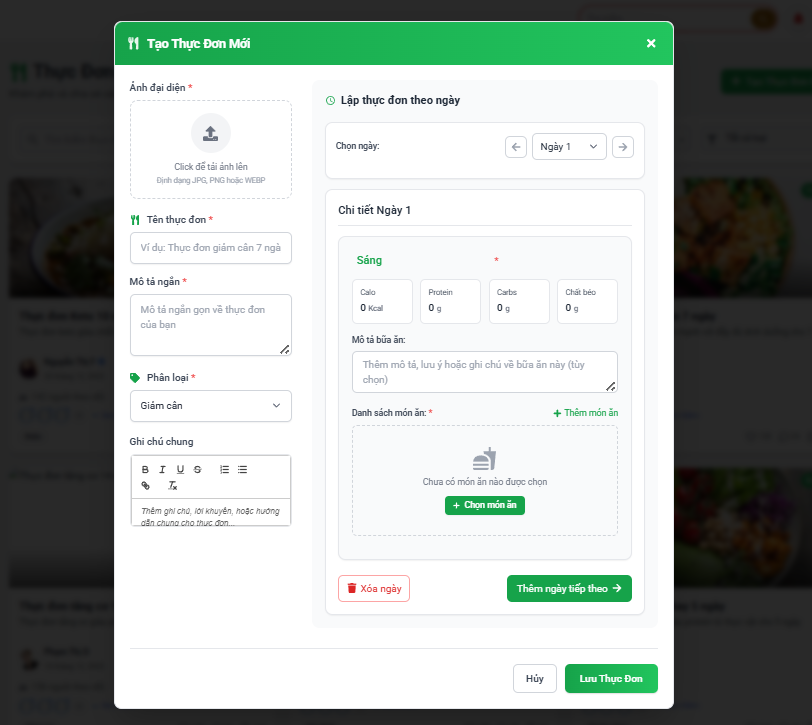
\includegraphics[width=0.8\textwidth]{Images/taothucdon.jpg}
    \vspace{1.5em}
    \caption{Giao diện trang tạo thực đơn}
    \label{fig:ui_create_meal}
\end{figure}

\subsection{Giao Diện Trang Chi Tiết Thực Đơn}
\label{subsec:impl_ui_meal_detail}
Hiển thị chi tiết một thực đơn, bao gồm danh sách ngày, món ăn, công thức, và phần tương tác (thả tim, bình luận, tham gia),.... Phân trang được áp dụng cho thực đơn dài.

\begin{figure}[H]
    \centering
    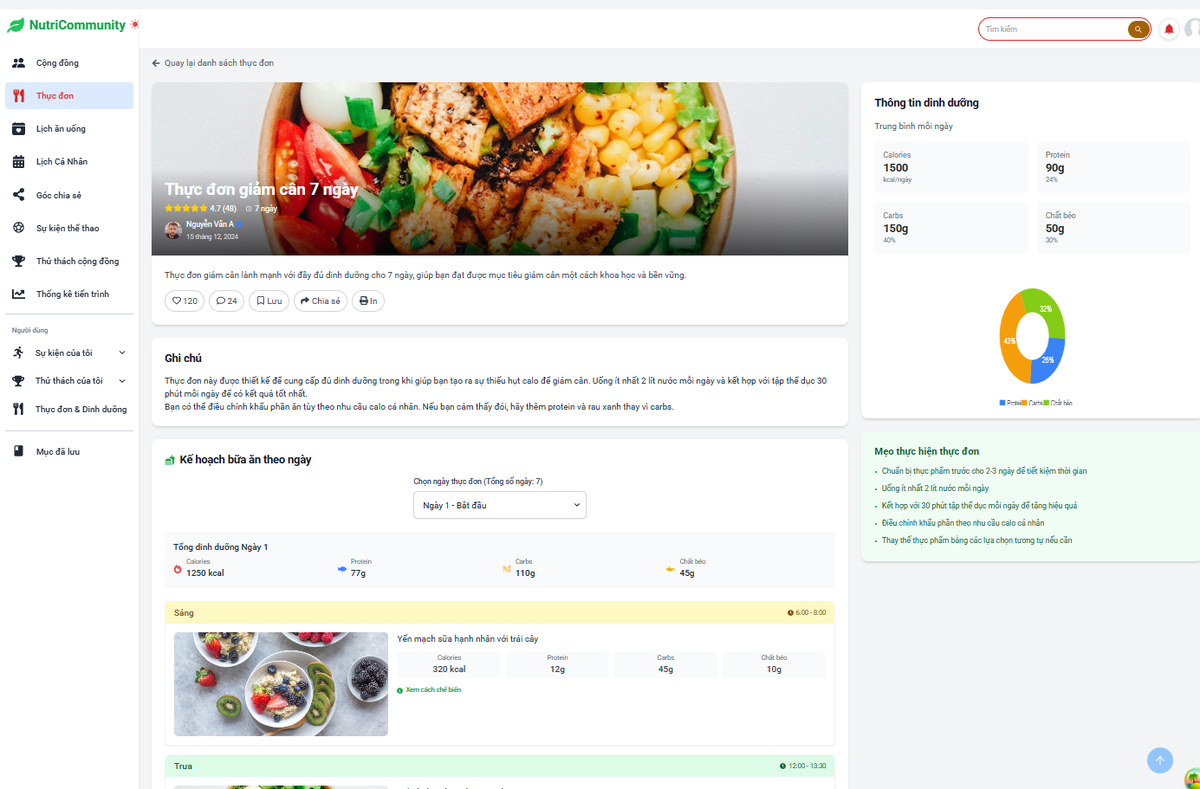
\includegraphics[width=0.8\textwidth]{Images/chitietthucdon.jpg}
    \vspace{1.5em}
    \caption{Giao diện trang chi tiết thực đơn}
    \label{fig:ui_meal_detail}
\end{figure}

\subsection{Giao Diện Trang Quản Lý Thực Đơn Của Tôi}
\label{subsec:impl_ui_my_meal}
Cho phép người dùng xem, chỉnh sửa, hoặc xóa các thực đơn đã tạo, hỗ trợ quản lý kế hoạch ăn uống cá nhân.

\begin{figure}[H]
    \centering
    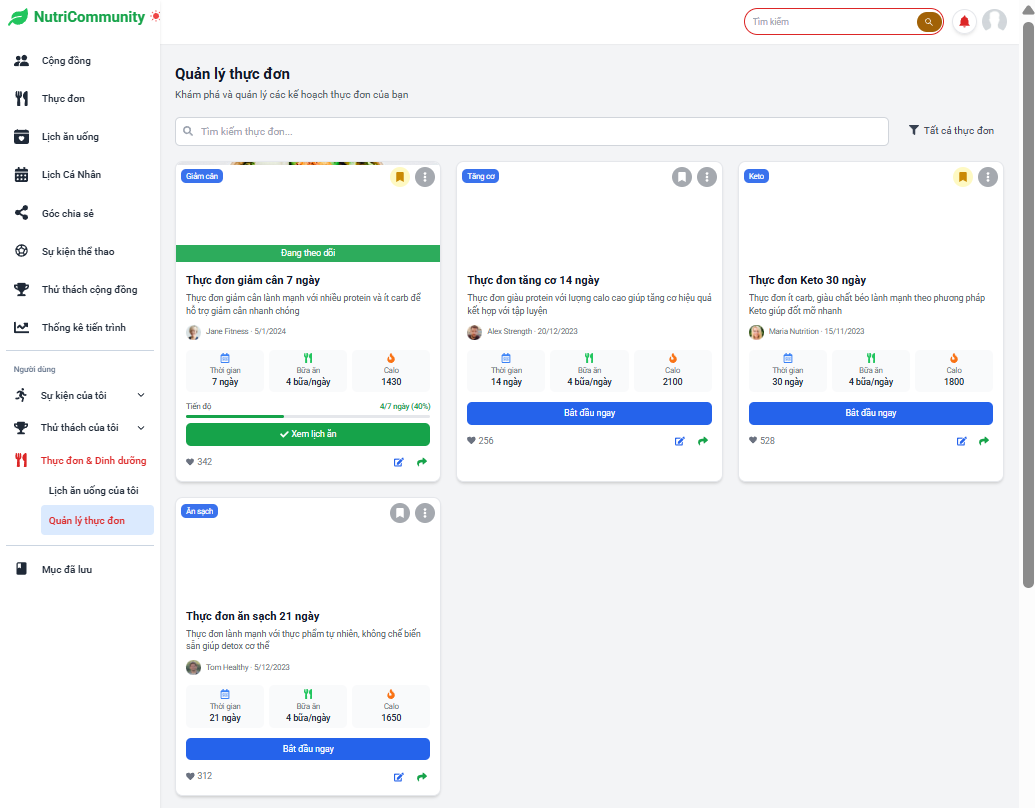
\includegraphics[width=0.8\textwidth]{Images/quanlythucdon.jpg}
    \vspace{1.5em}
    \caption{Giao diện trang quản lý thực đơn của tôi}
    \label{fig:ui_my_meal}
\end{figure}

\subsection{Giao Diện Trang Lịch Ăn Uống Của Tôi}
\label{subsec:impl_ui_my_schedule}
Hiển thị lịch ăn uống cá nhân, cho phép người dùng theo dõi các thực đơn đang thực hiện, kèm nhắc nhở nếu có.

\begin{figure}[H]
    \centering
    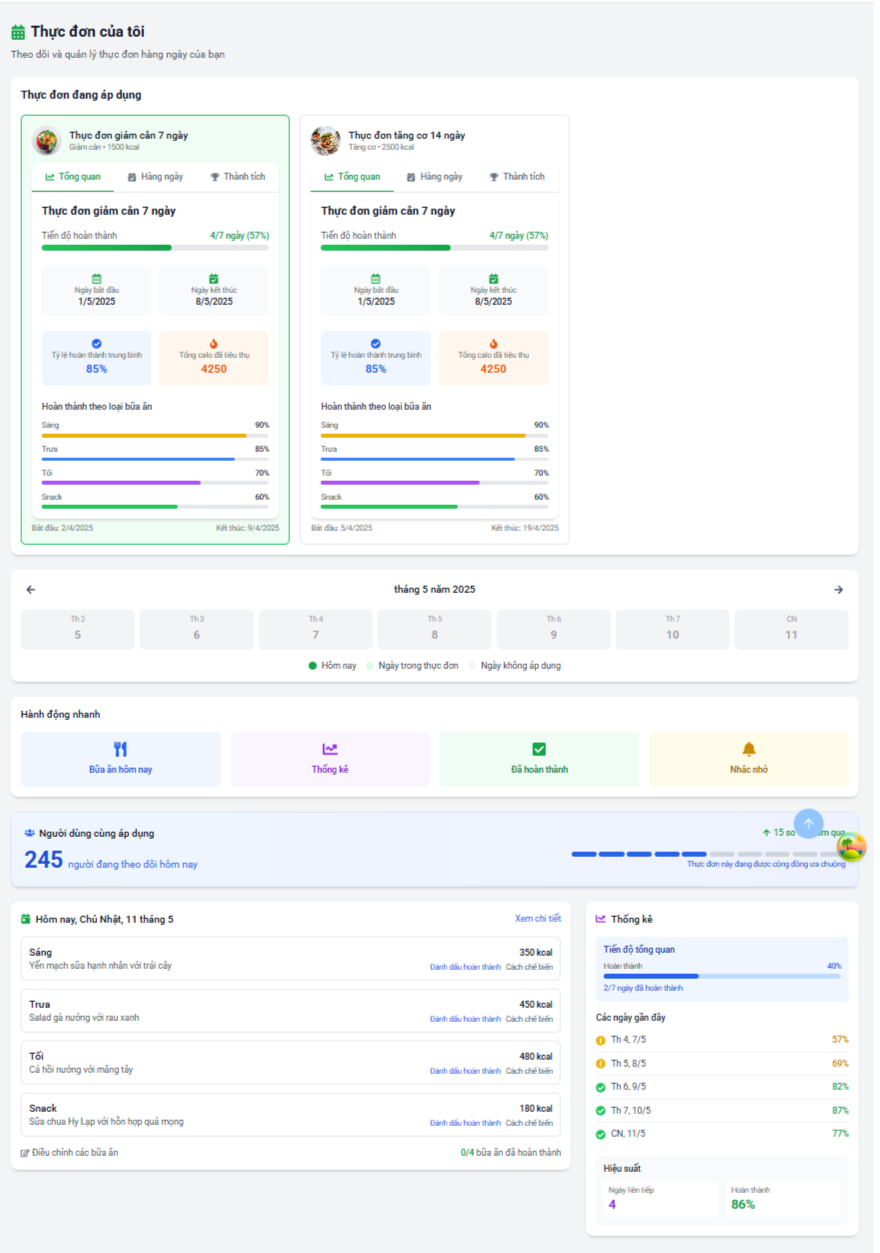
\includegraphics[width=0.8\textwidth]{Images/thucdoncuatoi.jpg}
    \vspace{1.5em}
    \caption{Giao diện trang lịch ăn uống của tôi}
    \label{fig:ui_my_schedule}
\end{figure}
\newpage
\section{Nhóm Tính Năng Sự Kiện Thể Thao}
\label{sec:impl_sport_event}

Nhóm tính năng sự kiện thể thao cho phép người dùng tạo, tham gia, và quản lý các sự kiện thể thao, tăng cường tương tác cộng đồng và động lực vận động.

\subsection{Giao Diện Trang Danh Sách Sự Kiện Thể Thao}
\label{subsec:impl_ui_sport_event_list}
Hiển thị danh sách các sự kiện thể thao, hỗ trợ tìm kiếm và lọc theo thể loại, loại sự kiện.

\begin{figure}[H]
    \centering
    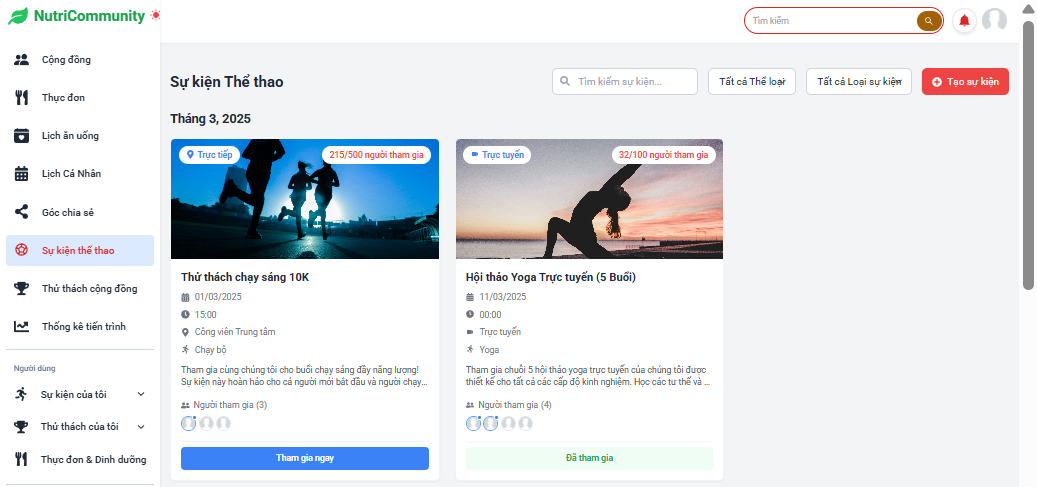
\includegraphics[width=0.8\textwidth]{Images/sukienthethao.jpg}
    \vspace{1.5em}
    \caption{Giao diện trang danh sách sự kiện thể thao}
    \label{fig:ui_sport_event_list}
\end{figure}

\subsection{Giao Diện Trang Tạo Sự Kiện Thể Thao}
\label{subsec:impl_ui_create_sport_event}
Cung cấp giao diện để người dùng nhập thông tin sự kiện như tên, thời gian, địa điểm, và mô tả,... Hỗ trợ thêm hình ảnh minh họa.

\begin{figure}[H]
    \centering
    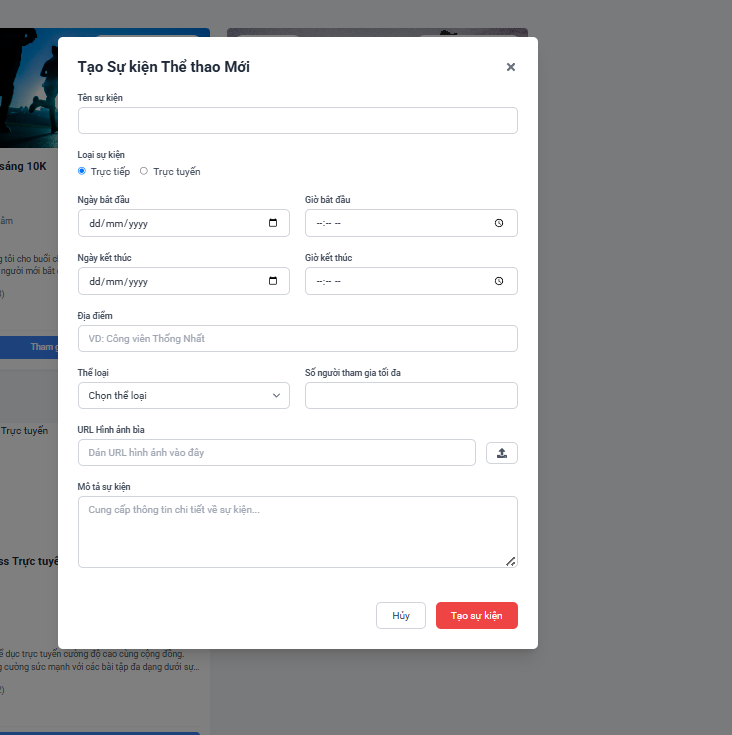
\includegraphics[width=0.8\textwidth]{Images/taosukienthethao.jpg}
    \vspace{1.5em}
    \caption{Giao diện trang tạo sự kiện thể thao}
    \label{fig:ui_create_sport_event}
\end{figure}

\subsection{Giao Diện Trang Chi Tiết Sự Kiện Thể Thao}
\label{subsec:impl_ui_sport_event_detail}
Hiển thị chi tiết một sự kiện, bao gồm thông tin, danh sách người tham gia, bài đăng cộng đồng, và lịch buổi học (đối với sự kiện trực tiếp).

\begin{figure}[H]
    \centering
    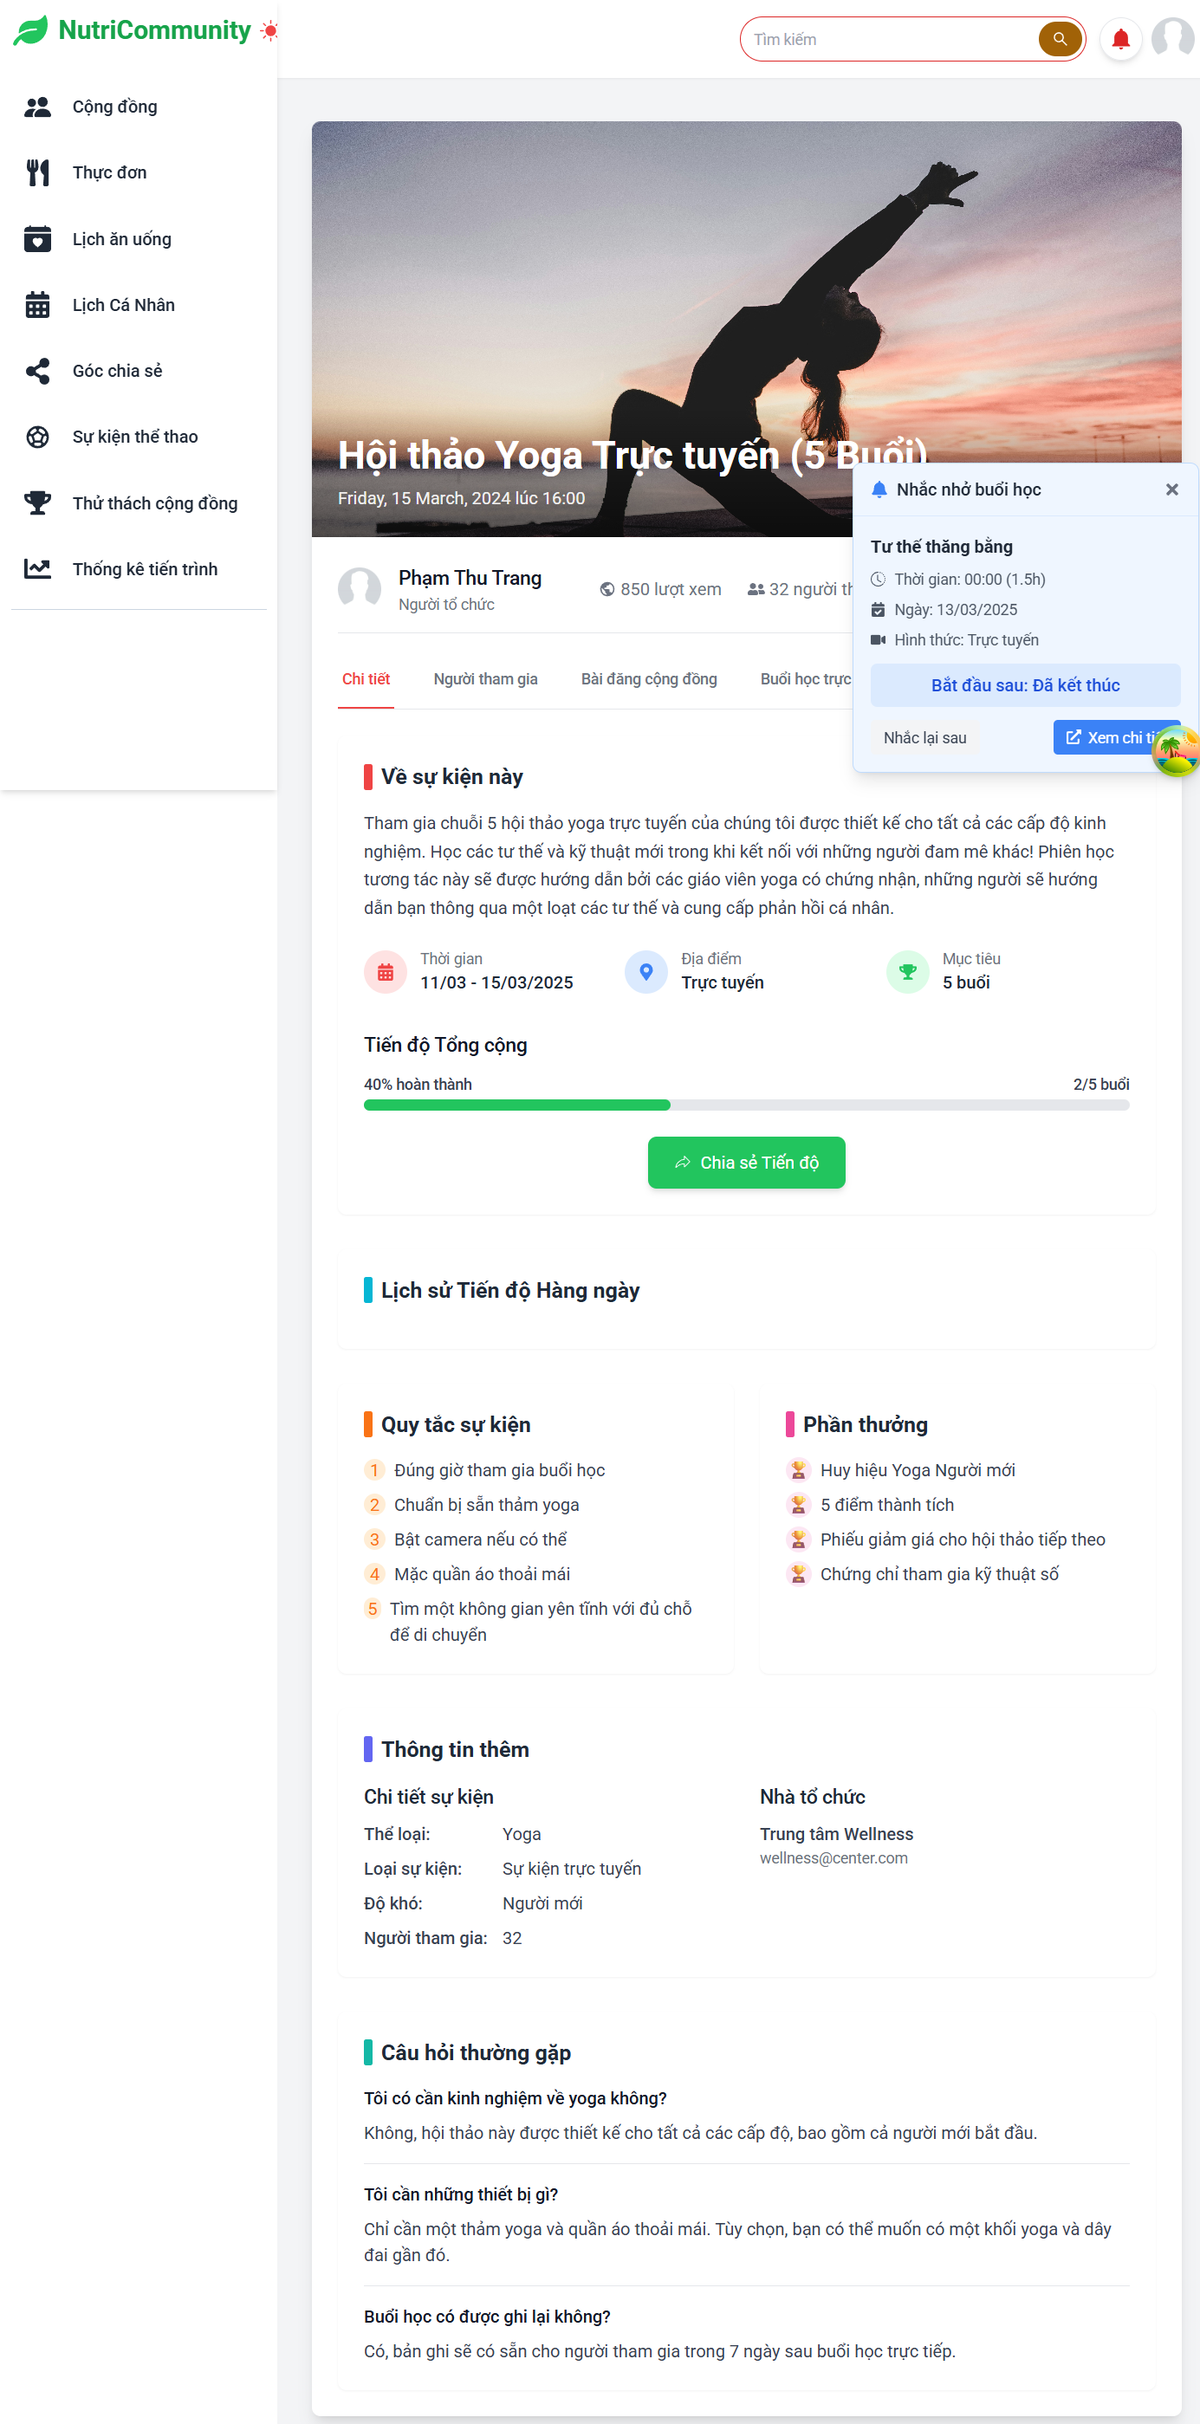
\includegraphics[width=0.8\textwidth]{Images/chitiet.jpg}
    \vspace{1.5em}
    \caption{Giao diện trang chi tiết sự kiện thể thao}
    \label{fig:ui_sport_event_detail}
\end{figure}

\subsection{Giao Diện Người Tham Gia Sự Kiện Thể Thao}
\label{subsec:impl_ui_sport_event_participants}
Hiển thị danh sách người tham gia sự kiện, cho phép người dùng xem hồ sơ hoặc tương tác.

\begin{figure}[H]
    \centering
    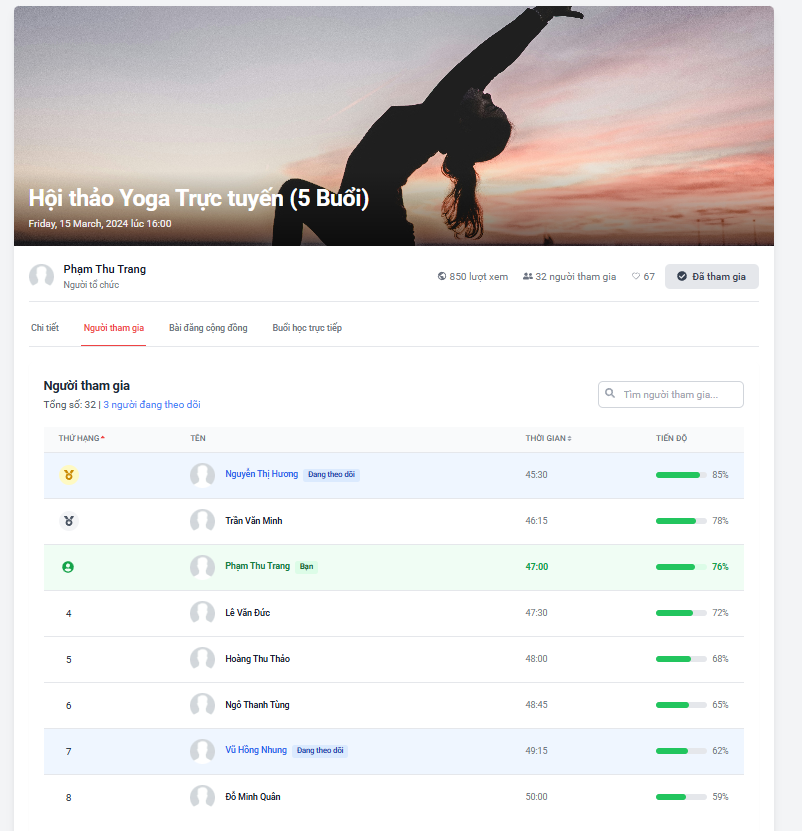
\includegraphics[width=0.8\textwidth]{Images/nguoithamgia.jpg}
    \vspace{1.5em}
    \caption{Giao diện danh sách người tham gia sự kiện thể thao}
    \label{fig:ui_sport_event_participants}
\end{figure}

\subsection{Giao Diện Bài Đăng Cộng Đồng Sự Kiện Thể Thao}
\label{subsec:impl_ui_sport_event_community}
Hiển thị các bài đăng liên quan đến sự kiện, hỗ trợ tương tác như thả tim, bình luận.

\begin{figure}[H]
    \centering
    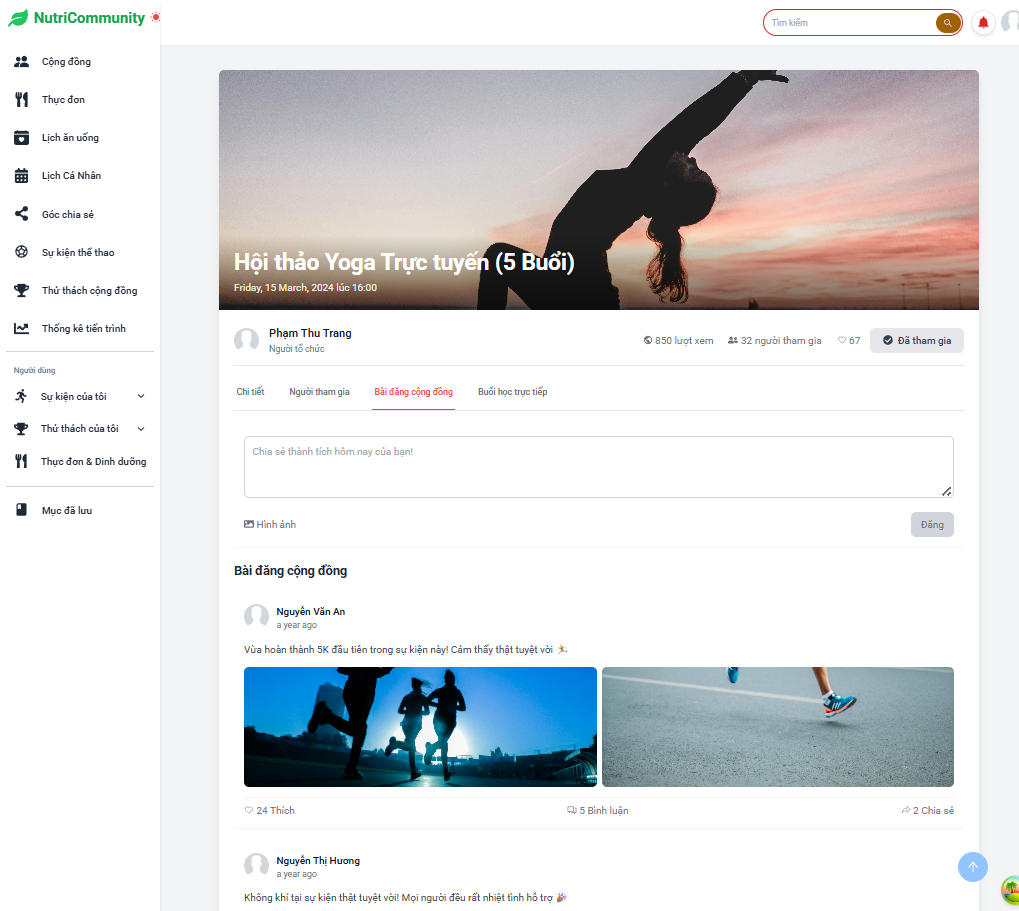
\includegraphics[width=0.8\textwidth]{Images/baidang.jpg}
    \vspace{1.5em}
    \caption{Giao diện cộng đồng trong trang chi tiết sự kiện thể thao}
    \label{fig:ui_sport_event_community}
\end{figure}

\subsection{Giao Diện Buổi Học Trực Tiếp Sự Kiện Thể Thao}
\label{subsec:impl_ui_sport_event_session}
Cung cấp giao diện để người dùng tham gia hoặc xem lịch các buổi học trực tiếp liên quan đến sự kiện.

\begin{figure}[H]
    \centering
    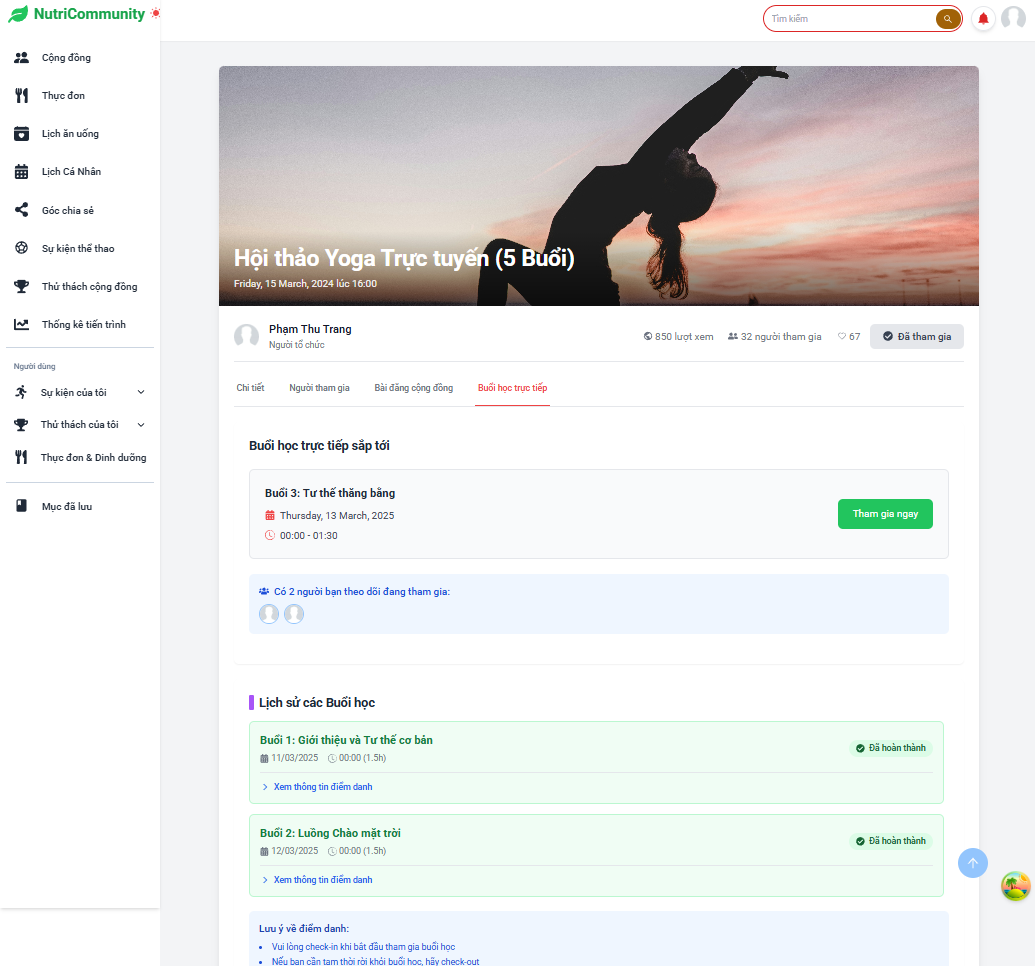
\includegraphics[width=0.8\textwidth]{Images/buoihoc.jpg}
    \vspace{1.5em}
    \caption{Giao diện buổi học trực tiếp sự kiện thể thao}
    \label{fig:ui_sport_event_session}
\end{figure}

\begin{figure}[H]
    \centering
    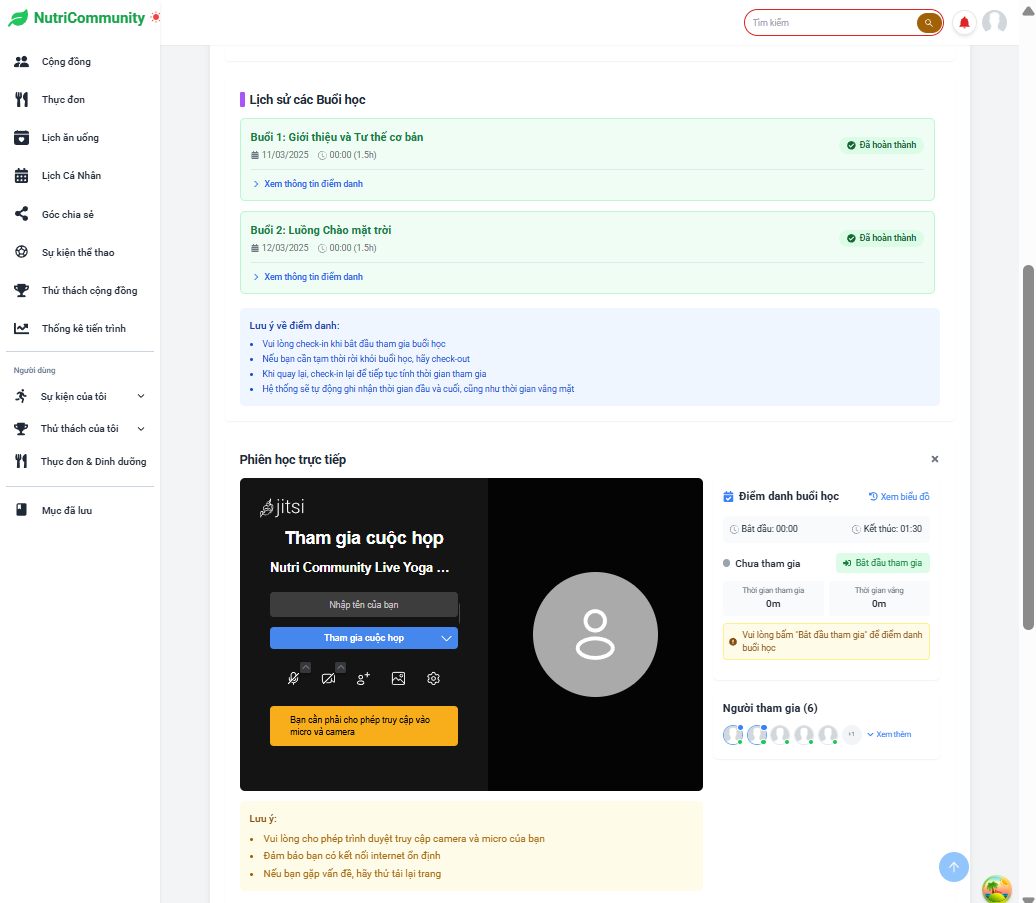
\includegraphics[width=0.8\textwidth]{Images/buoihoc2.jpg}
    \vspace{1.5em}
    \caption{Giao diện tham gia buổi học trực tiếp sự kiện thể thao}
    \label{fig:ui_sport_event_session_join}
\end{figure}

\subsection{Giao Diện Danh Sách Sự Kiện Thể Thao Đang Tham Gia}
\label{subsec:impl_ui_sport_event_active}
Hiển thị danh sách các sự kiện thể thao người dùng đang tham gia, hỗ trợ quản lý và theo dõi tiến độ.

\begin{figure}[H]
    \centering
    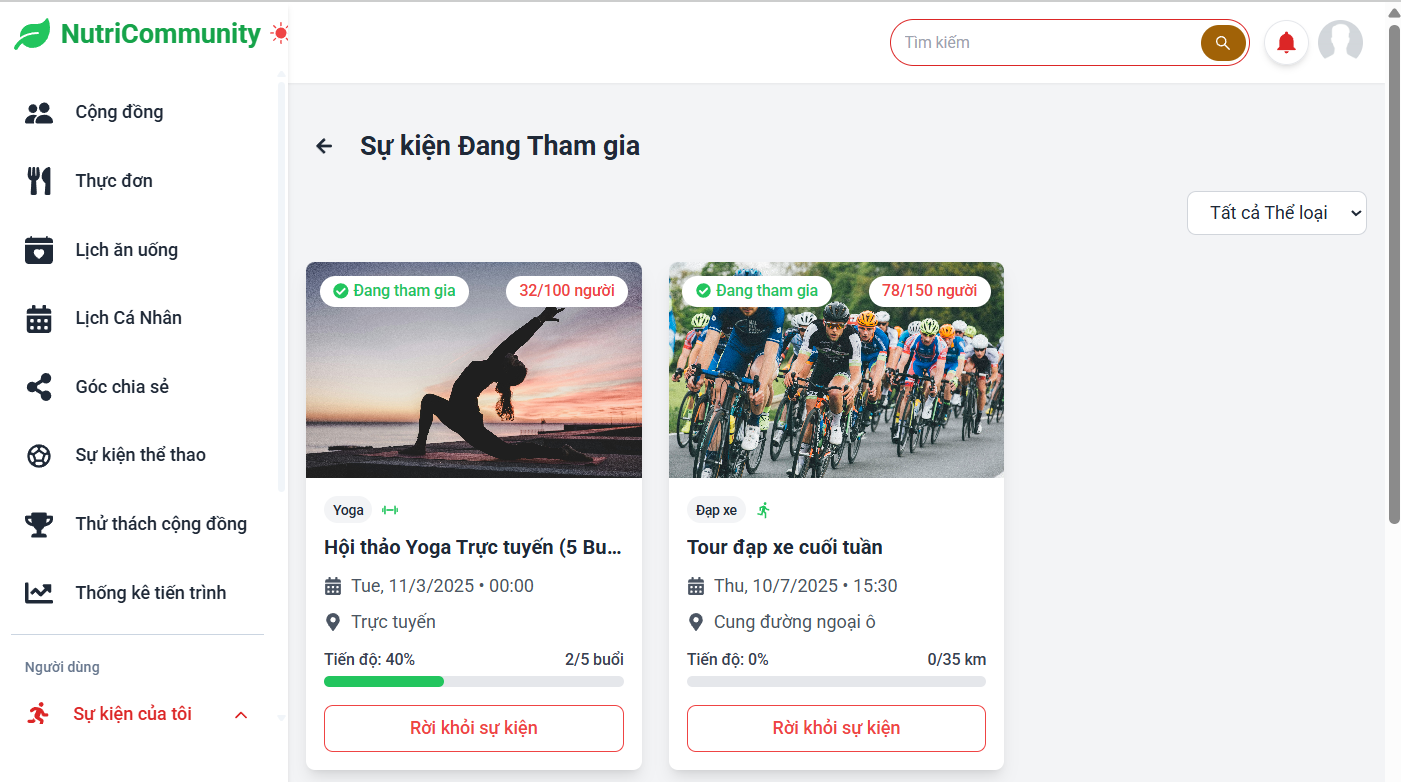
\includegraphics[width=0.8\textwidth]{Images/sukiendangthamgia.jpg}
    \vspace{1.5em}
    \caption{Giao diện danh sách sự kiện thể thao đang tham gia}
    \label{fig:ui_sport_event_active}
\end{figure}

\subsection{Giao Diện Lịch Sử Sự Kiện Thể Thao Đã Tham Gia}
\label{subsec:impl_ui_sport_event_history}
Hiển thị lịch sử các sự kiện thể thao người dùng đã tham gia, hỗ trợ xem lại thông tin và thành tích.

\begin{figure}[H]
    \centering
    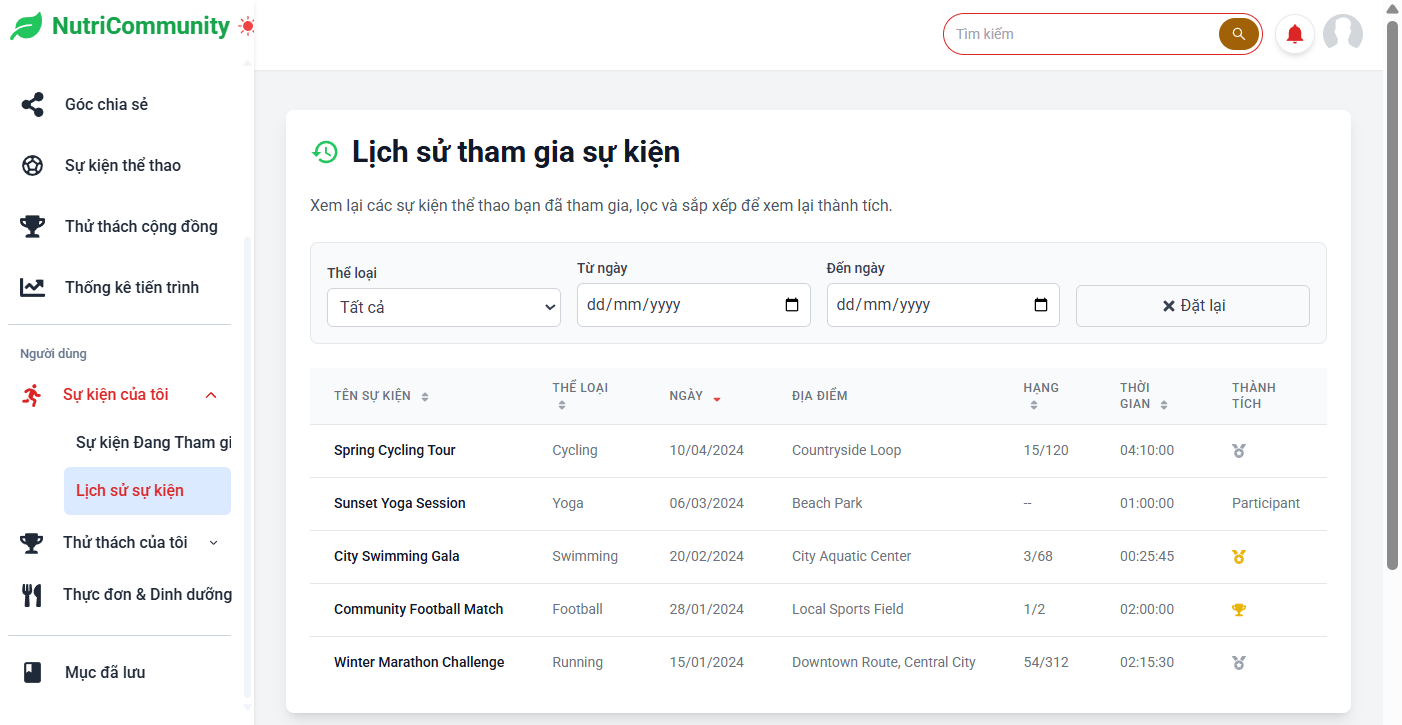
\includegraphics[width=0.8\textwidth]{Images/lichsusukien.jpg}
    \vspace{1.5em}
    \caption{Giao diện lịch sử sự kiện thể thao đã tham gia}
    \label{fig:ui_sport_event_history}
\end{figure}
\newpage
\section{Nhóm Tính Năng Thử Thách Cộng Đồng}
\label{sec:impl_challenge}

Nhóm tính năng thử thách cộng đồng khuyến khích người dùng tham gia các hoạt động lành mạnh thông qua các thử thách cá nhân hoặc nhóm, tăng tính kết nối và động lực.

\subsection{Giao Diện Danh Sách Thử Thách Cộng Đồng}
\label{subsec:impl_ui_challenge_list}
Hiển thị danh sách các thử thách cộng đồng, hỗ trợ tìm kiếm và lọc theo loại thử thách hoặc thời gian.

\begin{figure}[H]
    \centering
    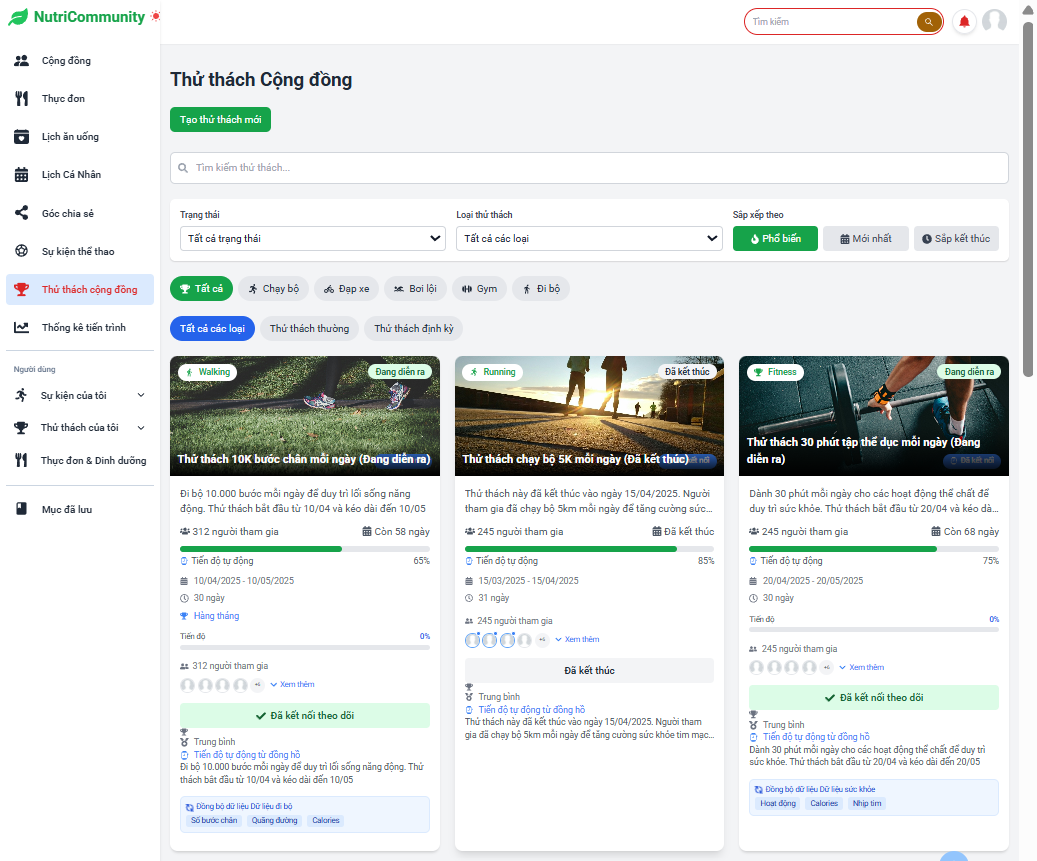
\includegraphics[width=0.8\textwidth]{Images/thuthachcongdong.jpg}
    \vspace{1.5em}
    \caption{Giao diện danh sách thử thách cộng đồng}
    \label{fig:ui_challenge_list}
\end{figure}

\subsection{Giao Diện Chi Tiết Thử Thách Cộng Đồng}
\label{subsec:impl_ui_challenge_detail}
Hiển thị chi tiết một thử thách, bao gồm mục tiêu, thời gian, và danh sách người tham gia. Hỗ trợ tương tác cộng đồng.

\begin{figure}[H]
    \centering
    
\includegraphics[width=0.8\textwidth]{Images/chitietthuthach.jpg}
    \vspace{1.5em}
    \caption{Giao diện chi tiết thử thách cộng đồng}
    \label{fig:ui_challenge_detail}
\end{figure}

\subsection{Giao Diện Trang Tạo Thử Thách Cộng Đồng}
\label{subsec:impl_ui_create_challenge}
Cung cấp giao diện để người dùng tạo thử thách mới, nhập thông tin như tên, mô tả, và mục tiêu.

\begin{figure}[H]
    \centering
    
\includegraphics[width=0.8\textwidth]{Images/taothuthach.jpg}
    \vspace{1.5em}
    \caption{Giao diện trang tạo thử thách cộng đồng}
    \label{fig:ui_create_challenge}
\end{figure}

\subsection{Giao Diện Trang Lịch Sử Thử Thách}
\label{subsec:impl_ui_challenge_history}
Hiển thị danh sách các thử thách người dùng đã tham gia, hỗ trợ xem lại tiến độ và kết quả.

\begin{figure}[H]
    \centering
    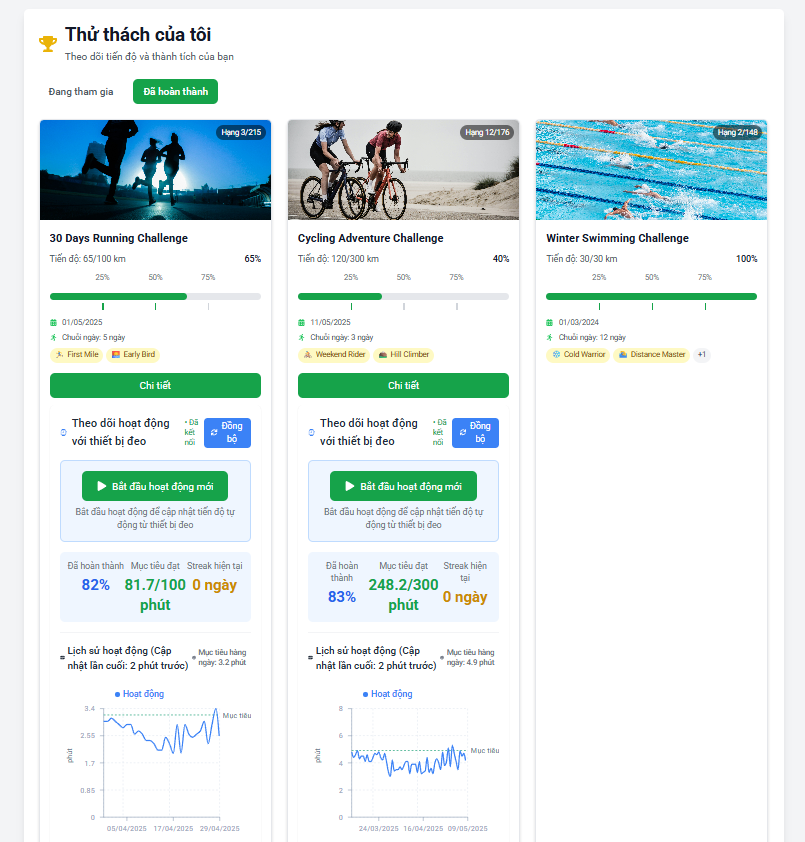
\includegraphics[width=0.8\textwidth]{Images/danhsachthuthachcuatoi.jpg}
    \vspace{1.5em}
    \caption{Giao diện lịch sử thử thách cộng đồng}
    \label{fig:ui_challenge_history}
\end{figure}